%!TEX TS-program = xelatex 
%!TEX TS-options = -output-driver="xdvipdfmx -q -E"
%!TEX encoding = UTF-8 Unicode
%
%  syllabus
%
%  Created by Mark Eli Kalderon on 2009-01-13.
%

\documentclass[11pt]{article} 

% Definitions
\newcommand\myauthor{Mark Eli Kalderon} 
\newcommand\mytitle{Oxford Philosophy of Perception:}
\newcommand\mysubtitle{Cook Wilson on Representation}

% Packages
\usepackage{url}
\usepackage{txfonts}
\usepackage{color}
\definecolor{myblue}{rgb}{0.8,0.8,1}

% Define discussion environment
\makeatletter\newenvironment{discussion}{%
   \noindent\begin{lrbox}{\@tempboxa}\begin{minipage}{\columnwidth}\setlength{\parindent}{1em}}{\end{minipage}\end{lrbox}%
   \colorbox{myblue}{\usebox{\@tempboxa}}
}\makeatother

% XeTeX
\usepackage[cm-default]{fontspec}
\usepackage{xltxtra,xunicode}
\defaultfontfeatures{Scale=MatchLowercase,Mapping=tex-text}
\setmainfont{Hoefler Text}
\setsansfont{Gill Sans}
\setmonofont{Inconsolata}

% Title Information
\title{\mytitle\\
\mysubtitle}
\author{\myauthor} 
\date{} % Leave blank for no date, comment out for most recent date

% PDF Stuff
\usepackage[plainpages=false, pdfpagelabels, bookmarksnumbered, backref, pdftitle={\mytitle}, pagebackref, pdfauthor={\myauthor}, xetex, colorlinks=true, citecolor=gray, linkcolor=gray, urlcolor=gray]{hyperref}

%%% BEGIN DOCUMENT
\begin{document}

% Title Page
\maketitle

% Layout Settings
\setlength{\parindent}{1em}

% Main Content

\begin{figure}[htbp]
	\centering
		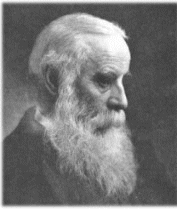
\includegraphics[scale=1]{../graphics/wilson.jpg}
	\caption{John Cook Wilson}
	\label{fig:wilson}
\end{figure}

\section{Preliminaries} % (fold)
\label{sec:preliminaries}

Cook Wilson begins with some interesting preliminary remarks. Let me mention, without elaborating, just two. Both concern, as we would put it, ordinary language philosophy. 

The first is a methodological observation. According to Cook Wilson, Stout exaggerates the difference between the philosopher and the plain man, but: ``As philosopher's we interrogate ourselves as plain men.'' 

The second concerns the difference between heat and color (or the difference between touch and sight, more generally). We speak of the sensation of heat but we never speak of the sensation of yellow. We feel hot but we do not feel yellow. On this basis, Cook Wilson concludes that talk of color sensations is not a commitment of common sense but is theoretically motivated (whether by psychology or philosophy). Later it emerges that this is a linguistic manifestation of a phenomenological difference. It is partly for this reason that Cook Wilson focuses on heat as opposed to color as a paradigm exemplar of a secondary quality.

\begin{discussion}
    Paul Snowdon queried the significance of Cook Wilson's linguistic observation. The absence of the verb ``feel'' in ordinary perceptual reports of color does not, by itself, mean that the perception of color involves no sensation. After all, we can \emph{have} sensations as well as \emph{feel} them. Perhaps the verb ``feel'' is restricted in its use to reporting certain types of sensations. The linguistic reflections are thus not decisive. However, I suspect that what \emph{is} decisive, at least by Cook Wilson's lights, is the phenomenological difference that the linguistic difference allegedly manifests.
\end{discussion}

% section preliminaries (end)

\section{Representation} % (fold)
\label{sec:representation}

Cook Wilson singles out for criticism Stout's claim that the sensations which mediate knowledge of secondary qualites do so only in so far as ``they represent, express, or stand for something other than themselves''.

Cook Wilson insists that talk of representation in philosophy is ``loose and treacherous'', a ``trap word'', and undertakes a ``critique'' of its meaning.

There are five main points:

A. First, perhaps the most fundamental issue consists in negative and positive claims about the nature of representation. The negative claim is that nothing is intrinsically representational: ``Nothing has \emph{meaning} in itself''. Presumably this was an effective point against those of his contemporaries who held that ideas are intrinsically representational. The positive claim is put as follows: ``Representation is our subjective act. \ldots\ It is \emph{we} who mean''. It is on these grounds that Cook Wilson criticizes Bradley's theory of judgment (\emph{Statement and Inference}, XIII, §§124-125). This thought, or something very much like it, independently animates McDowell in his discussion of Dennett, and Travis in his discussion of the representational theory of experience. While this is really the fundamental point, Cook Wilson doesn't stress it in his critique of Stout. Nor does he explicitly argue for it, either in the present letter or in the manuscript about Bradley's theory of judgement. Perhaps the thought is that in the absence of anything being intrinsically representational, the only fact that could make for representation essentially involves a subject.

\begin{discussion}
    Rory Madden observed that there are two ways in which the slogan ``It is \emph{we} who mean'' might be understood:
    \begin{itemize}
    	\item Perhaps representation is \emph{personal} in the sense that it belongs to a conscious subject.
    	\item Perhaps represenation is \emph{agential} in the sense that its the result of something a person does.
    \end{itemize}

    The distinction potentially bears on whether Cook Wilson's criticism generalizes to encompass, not only representative realism, but the representational theory of experience (understood \emph{not} as an explanatory hypothesis about the phenomenal character of experience of the kind that Harman endorses, but merely as the attribution to experience of representational content.) Perhaps, an agential conception of representation, if developed and sustained, would count against the representational theory of experience (but see McDowell's remarks about spontaneity); but it is unobvious that a personal conception of representation would. Experiences are, after all, states of a subject (contrast subpersonal states of a subject such as neurophysiological states). Perhaps that is enough to satisfy the constraints imposed by a personal conception of representation. The matter is unclear. It all depends on how much must be built into the notion of personal representation. If it is a more demanding notion, then more would have to be said in defense of it.
\end{discussion}

Without settling on a specific interpretation of the slogan ``It is \emph{we} who mean'', I will henceforth refer to the general class of views as \emph{personal} conceptions of representation.

B. Second, Cook Wilson draws a distinction between two natural relations that ground different notions of representation.
\begin{itemize}
	\item \( A \) may represent \( B \) because \( A \) resembles \( B \) (\emph{mimetic representation})
	\item \( A \) may represent \( B \) because the existence of \( A \) necessitates the existence of \( B \) (\emph{factive representation})
\end{itemize}

\begin{discussion}
    Paul Snowdon wondered how this could be consistent with the fundamental point that it is \emph{we} who mean, since these are natural relations which can obtain independently of a subject. The distinction could not consist thereby in two analyses of different notions of representation, since the resulting conceptions of representation would be impersonal. Perhaps mimesis and necessary covariation are natural relations that merely \emph{incline} us to represent things by means of them. Perhaps they are merely relations whose obtaining can be exploited by a person's representational ends. Something like this is suggested by the following passage:
    \begin{quote}
    	It is we who make the weeping willow a symbol of sorrow. There may of course be something in the object which prompts us to give it a meaning, e.g., the resemblance of the weeping willow to a human figure bowed over in the attitude of grief. But the willow in itself can neither `mean' grief, nor `represent' nor `stand for' nor `express' grief. \emph{We} do all that. (\emph{Statement and Inference}, 770)
    \end{quote}
    The resemblance of the weeping willow to a human figure bowed over in the attitude of grief is thus not \emph{sufficient} for the former to represent the latter (and so mimesis is not an analysis of a kind of representation), though it may incline us to take the former to represent the latter.

    Paul Snowdon also wondered whether in taking personal representation as the fundamental notion, Cook Wilson was eliding the Gricean distinction between \emph{natural} and \emph{non-natural} meaning. The natural relations of mimesis and necessary covariation are, after all, candidates for being Gricean natural meanings, but Cook Wilson seems to deny that they are representations of any sort in the absence of use by a person.

    If all Grice means by natural meaning is an information-bearing state (in a sense of information that precludes misinformation), then \( A \)'s resembling or necesssarily covarying with \( B \) suffices for \( A \) to naturally mean \( B \). Cook Wilson's point would then be that these natural relations are insufficient for a notion of representation that leaves room for the possibility of error, of misinformation or misrepresentation.

    Paul Snowdon suggests that this dialectic reveals a lacuna in Cook Wilson's case. Perhaps representation \emph{in a particular sense} is personal and so liable to misrepresentation. But Cook Wilson is not acknowledging any restriction in the use of representation, but is singling out, without explicit justification, one sense of representation as fundamental.
\end{discussion}

C. Third, Cook Wilson emphasizes the symmetry of these relations. If \( A \) resembles \( B \) in some respect, \( B \) resembles \( A \) in that respect. If \( A \) necessarily covaries with \( B \), \( B \) necessarily covaries with \( A \). This undermines the asymmetry between Stout's talk of a sense-representation and what it represents. Or rather, if that asymmetry is sustained, this is evidence of a further assumption in play. Specifically, if \( A \) represents \( B \) without \( B \) representing \( A \) this is because \( A \) but not \( B \) is ``present to consciousness''.

One worry is whether Cook Wilson has specified the hidden assumption in a non-question-begging manner. At least by the lights of a representative realist such as Stout, shouldn't it rather be ``\emph{immediately} present to consciousness''? 

\begin{discussion}
	Lee Walters observes that in the specification (above and in Cook Wilson's text) of the natural relation involved in factive representation the relation is described as ``necessitation''. But there is a good sense of necessitation in which it is not symmetric. That's certainly true, but Cook Wilson's repeated emphasis on the symmetry of the relation is evidence that by ``necessitates'' he means the symmetric relation of necessary covariation. It was also observed that the factive nature of the relation does not require the modal element nor does the symmetry of the relation require that it be factive (it might be a symmetrical statistical relation of some sort).

	Paul Snowdon points out how the personal conception of representation is at work here in Cook Wilson's reflections on symmetry. Suppose that Stout is working with an impersonal notion of representation (though he shouldn't, at least by Cook Wilson's lights). If Stout is working with an impersonal notion of representation then the the external world could (impersonally) represent the sensation, it is just not a relation that anyone could exploit.
\end{discussion}


D. Fourth, Cook Wilson doubts that the relevant notion of representation could be mimetic. Two arguments:

1. The Berkelean argument: Only a sensation can resemble a sensation. So if representation were mimetic, the plain man would be guilty of the ``flagrant absurdity''.

2. In feeling the shape of a thing, we have feelings distinct from extension and yet is through these feelings that we become aware of the thing's shape. Here tactile sensation mediates our knowledge of extension. But talk of mediation implies that that the tactile sensations differ from extension and so they cannot be representative by means of resemblance.

There is a potential lacuna in this argument. That tactile sensation mediates our knowledge of extension may establish that sensation and extension are numerically distinct, but it does not follow from numerical distinctness that the sensation could not mimetically represent extension. To establish that, we would need the stronger claim that sensation and extension differ in kind. If sensation and extension are unlike in kind then there would be no mimetic relation in virtue of which a person could represent the latter by the former.

It is unlikely that Cook Wilson conflates numerical distinction with distinction in kind since he repeatedly emphasizes this difference in other contexts and commends due attention to it to Stout. So what bridges the gap in the argument? Is Cook Wilson simply helping himself to the Berkelean argument (in which case we do not have two arguments but two variants of the same argument.)

\begin{discussion}
	Paul Snowdon suggests that what bridges the gap is a phenomenological claim---that there is nothing in sensation that is spatial. Perhaps the following is the statement of the alleged phenomenological claim:
	\begin{quote}
		Here (in felt extension) we seem to recognize in feeling round the surfaces and edges of a die (e.g.) that we have certain feelings quite different from the extension, and yet that it is somehow \emph{through} these feelings that we become aware of the extension. (\emph{Statement and Inference}, 771)
	\end{quote}
	But if the argument turns on this phenomenological claim, why should Stout accept it? Perhaps Cook Wilson thinks that this is the closest and most specific claim about the relevant phenomenology in the area, and that it is simply not going to do for Stout's purposes.
\end{discussion}


E. Fifth, if we consider sensations as representative this must be so either on the grounds of likeness or covariation with extension. We must already be acquainted with the likeness or know the covariation. But this is impossible if the mediation of our knowledge of extension by sensation means that we depend on such sensations for our knowledge of extension.

How plausible is the operative epistemological premise? Advocates of certain forms of naturalized semantics, such as Fodor's correlational psychosemantics, would deny any such epistemic assumption. So would reliabilists like Goldman who maintain that what confers justification on belief is that it is formed by a reliable belief forming mechanism, not that we know that it is so formed. Are they justified in doing so? What does this tell us about Cook Wilson's argument?

I suspect that here too, the personal conception of representation is at work, at least implicitly. The hypothesis is that the restriction that we should know of the relevant natural relations flows form the thought that it is only if we know of such relations that we could exploit them for our representational ends.

% section representation (end)
\end{document}
